\section{Proposal of a Solution}

The proposal: An atomic data management system utilizing a smartwatch to take advantage of faster and more instantaneous data input.
The here proposed solution features a \gls{pims} supporting relationships
between bits of information. Since the proposed solution does not store
information sequentially but relationally, the reorganization of existing
information is possible without changing the information itself.

\subsection{Atomic Data}

\begin{center}
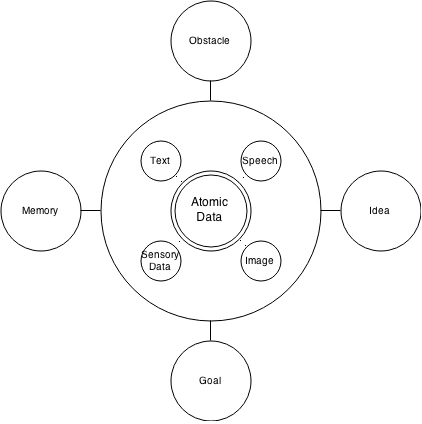
\includegraphics[width=0.9\linewidth]{00_resources/atomic_data.png}
\end{center}

Atomic data is in this case defined as small user-entered bits of information which do not have to adhere to any standard.
On the right, a small illustration, the types of data the application supports can be seen.

\subsection{Data Input Methods}

\begin{center}
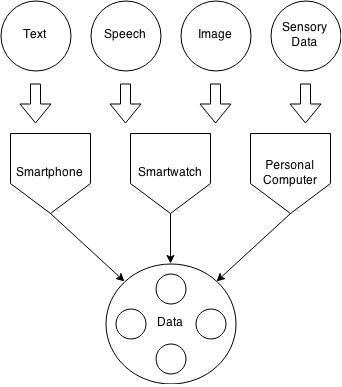
\includegraphics[width=0.9\linewidth]{00_resources/input_methods.png}
\end{center}

The data pieces can be inserted into the database utilizing the available input devices such as smartphones and smartwatches. Of course, a smartwatch can only capture little bits of information while a laptop can capture huge amounts. However, a smartwatch can be used instantly for capturing a piece of data while a laptop has to be prepared for capturing.

\subsection{Organization of Data}

Previously inserted atomic bits of data can be organized using a variety of models which are not all specified in this document. The more obvious ones are folders and labels as well as relationships between atomic data which can then be visualized as maps and radial relationship diagrams.

\subsubsection{Relationships}

\begin{center}
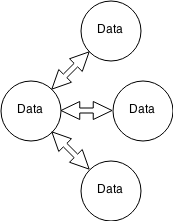
\includegraphics[width=0.5\linewidth]{00_resources/data_relationships.png}
\end{center}

Data can be organized in relationships where each relationship has two data atoms and a set of attributes such as the direction or the cardinality of the relationship. Relationships between data atoms can be displayed either on a map or on a radial graph showing only closest relations.

\subsubsection{Labels}

\begin{center}
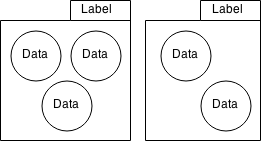
\includegraphics[width=0.5\linewidth]{00_resources/data_labels.png}
\end{center}

Data atoms can be grouped in labels or folders where each label optionally has attributes such as color.

\subsubsection{Timeline}

\begin{center}
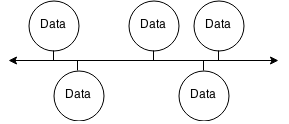
\includegraphics[width=0.5\linewidth]{00_resources/data_timeline.png}
\end{center}

Data atoms can be ordered by time either manually specified or by the creation time of the data atom itself.

\subsubsection{Matrix}

\begin{center}
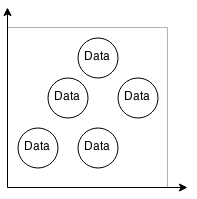
\includegraphics[width=0.5\linewidth]{00_resources/data_matrix.png}
\end{center}

Data atoms can be part of a two-dimensional matrix which can then be visualized.
